\documentclass[11pt,a4paper]{article}

\usepackage[a4paper, top=2.5cm, bottom=2.5cm, left=2.5cm, right=2.5cm]{geometry}
\usepackage[T1]{fontenc}
\usepackage[utf8]{inputenc}
\usepackage{mathptmx}
\usepackage{setspace}
\usepackage{parskip}
\usepackage{titlesec}
\usepackage{fancyhdr}
\usepackage{booktabs}
\usepackage{tabularx}
\usepackage{longtable}
\usepackage{array}
\usepackage{enumitem}
\usepackage{hyperref}
\usepackage{lastpage}
\usepackage{needspace}
\usepackage{tikz}
\usepackage{float}
\usepackage{caption}
\usetikzlibrary{shapes.geometric, arrows.meta, positioning, fit, backgrounds}

\raggedbottom
\hypersetup{colorlinks=false, hidelinks}

\setstretch{1.07}
\setlength{\parskip}{4pt}
\setlength{\parindent}{0pt}
\setlength{\headheight}{14pt}

\titleformat{\section}{\large\bfseries}{}{0em}{}
\titleformat{\subsection}{\normalsize\bfseries}{}{0em}{}
\titleformat{\subsubsection}{\normalsize\itshape}{}{0em}{}
\titlespacing*{\section}{0pt}{14pt}{5pt}
\titlespacing*{\subsection}{0pt}{9pt}{3pt}
\titlespacing*{\subsubsection}{0pt}{6pt}{2pt}

\setlist[itemize]{leftmargin=1.5em, itemsep=1pt, topsep=2pt, parsep=0pt}
\setlist[enumerate]{leftmargin=1.5em, itemsep=1pt, topsep=2pt, parsep=0pt}

\pagestyle{fancy}
\fancyhf{}
\renewcommand{\headrulewidth}{0.4pt}
\fancyhead[L]{\small Requirements Engineering Assignment 4 \quad ParcelResolve}
\fancyfoot[C]{\small Page \thepage\ of \pageref{LastPage}}

% TikZ styles for diagrams
\tikzset{
  state/.style={rectangle, rounded corners=3pt, draw=black, fill=white,
                text width=3.8cm, align=center, minimum height=0.7cm, font=\small},
  decision/.style={diamond, draw=black, fill=white,
                   text width=2.2cm, align=center, aspect=1.8, font=\small\itshape},
  invalid/.style={rectangle, rounded corners=3pt, draw=black, fill=black!10,
                  text width=2.8cm, align=center, minimum height=0.6cm, font=\small},
  valid/.style={rectangle, rounded corners=3pt, draw=black, fill=black!5,
                text width=2.8cm, align=center, minimum height=0.6cm, font=\small},
  reject/.style={rectangle, draw=black, fill=black!20,
                 text width=1.8cm, align=center, minimum height=0.6cm, font=\small},
  arrow/.style={-{Stealth[length=5pt]}, thin},
  darrow/.style={-{Stealth[length=5pt]}, thin, dashed},
}

\begin{document}

% ============================================================
% TITLE BLOCK
% ============================================================
\begin{center}
{\large\bfseries Requirements Engineering Assignment 4}\\[0.2cm]
{\Large\bfseries ParcelResolve}\\[0.15cm]
{\large Model-Based Validation Report}\\[0.4cm]
\begin{tabular}{ll}
Group Name: & Varun \& Thanh \\
Students:   & Varun Ganesh Sondur \\
            & Pham Thanh \\
\end{tabular}
\end{center}
\vspace{4pt}\hrule\vspace{8pt}

% ============================================================
% SECTION 1 — INTRODUCTION
% ============================================================
\section*{1.\enspace Introduction}

\subsection*{1.1\enspace Purpose}

This report is our Model-Based Validation of the ParcelResolve requirements specification from Assignment~3. Instead of reviewing each requirement on its own, we checked the requirements against a behavioural model of the incident lifecycle, to see whether they describe a resolution process that actually hangs together.

The validation looks at: valid states and transitions; normal and alternative resolution paths; exceptional situations; the conditions for moving between lifecycle stages; the conditions for resolution verification and closure; and anything missing, contradictory, ambiguous, or incomplete.

\subsection*{1.2\enspace Requirements Under Validation}

The validation uses the requirements specification from Assignment~3:

\begin{itemize}
  \item \textbf{28 Functional Requirements:} FR-01–FR-28
  \item \textbf{16 Non-Functional Requirements:} NFR-01–NFR-16
\end{itemize}

That is \textbf{44 requirements} in total. The functional requirements cover incident initiation, classification, information management, workflow, actions and responsibility, evidence, monitoring, escalation, customer communication, resolution verification, closure, and operational insights. The non-functional requirements cover performance, capacity, availability, reliability, security, access control, auditability, usability, maintainability, integration, and observability.

\subsection*{1.3\enspace Validation Approach}

Model-Based Validation checks whether the requirements are consistent with an explicit model of expected system behaviour. Our process was:

\begin{center}
\small
Assignment~3 Requirements $\rightarrow$ Behavioural Model $\rightarrow$ Requirement-to-Model Mapping $\rightarrow$ Model Scenarios and Transitions $\rightarrow$ Validation Questions $\rightarrow$ Findings and Requirement Refinement
\end{center}

The model is not meant to describe implementation architecture. It describes how we expect an incident to move through the ParcelResolve resolution process.

% ============================================================
% SECTION 2 — BEHAVIOURAL MODEL
% ============================================================
\section*{2.\enspace Behavioural Model}

\subsection*{2.1\enspace Model Objective}

The model represents the lifecycle of a parcel incident from detection or reporting until verified resolution and closure. The main lifecycle established in Assignment~2 is:

\begin{center}
\textbf{Detect $\rightarrow$ Understand $\rightarrow$ Act $\rightarrow$ Monitor $\rightarrow$ Verify Resolution $\rightarrow$ Close}
\end{center}

The model extends this lifecycle with alternative and exceptional paths where the Assignment~3 requirements need them.

\subsection*{2.2\enspace Main States}

\subsubsection*{Detect}
The incident enters ParcelResolve after a parcel problem is detected by an integrated operational system or reported by a customer or customer-service channel. Relevant requirements: FR-01, FR-02, FR-03.

\subsubsection*{Understand}
The system gathers and maintains information required to understand the incident, including classification, incident information, current status, history, and evidence. Relevant requirements: FR-04–FR-08, FR-14–FR-16.

\subsubsection*{Act}
The applicable resolution workflow is selected and required actions are created, assigned, and tracked. Relevant requirements: FR-09–FR-13.

\subsubsection*{Monitor}
Open incidents and their actions are monitored for deadlines, overdue conditions, status changes, and relevant new information. Relevant requirements: FR-17, FR-18.

\subsubsection*{Escalation}
An incident may require escalation when configured conditions are met. Escalation can result in reassignment, priority changes, notification, or a workflow change. Relevant requirements: FR-19, FR-20.

\subsubsection*{Verify Resolution}
The system checks whether the applicable resolution conditions have actually been satisfied. Completing an action is not by itself enough to close an incident. Relevant requirement: FR-24.

\subsubsection*{Close}
The incident is closed only after the applicable resolution conditions have been verified. The resolution outcome and closure information are recorded. Relevant requirements: FR-25, FR-26.

\subsection*{2.3\enspace Supporting Behaviour}

Some requirements support several lifecycle states rather than one individual state: customer communication (FR-21–FR-23); operational insights (FR-27–FR-28); and auditability and quality constraints (NFR-01–NFR-16). We validated these against individual states and across the lifecycle as a whole.

% ============================================================
% SECTION 3 — MAIN BEHAVIOURAL MODEL
% ============================================================
\section*{3.\enspace Main Behavioural Model}

The following model represents the main incident-resolution flow.

\begin{figure}[H]
\centering
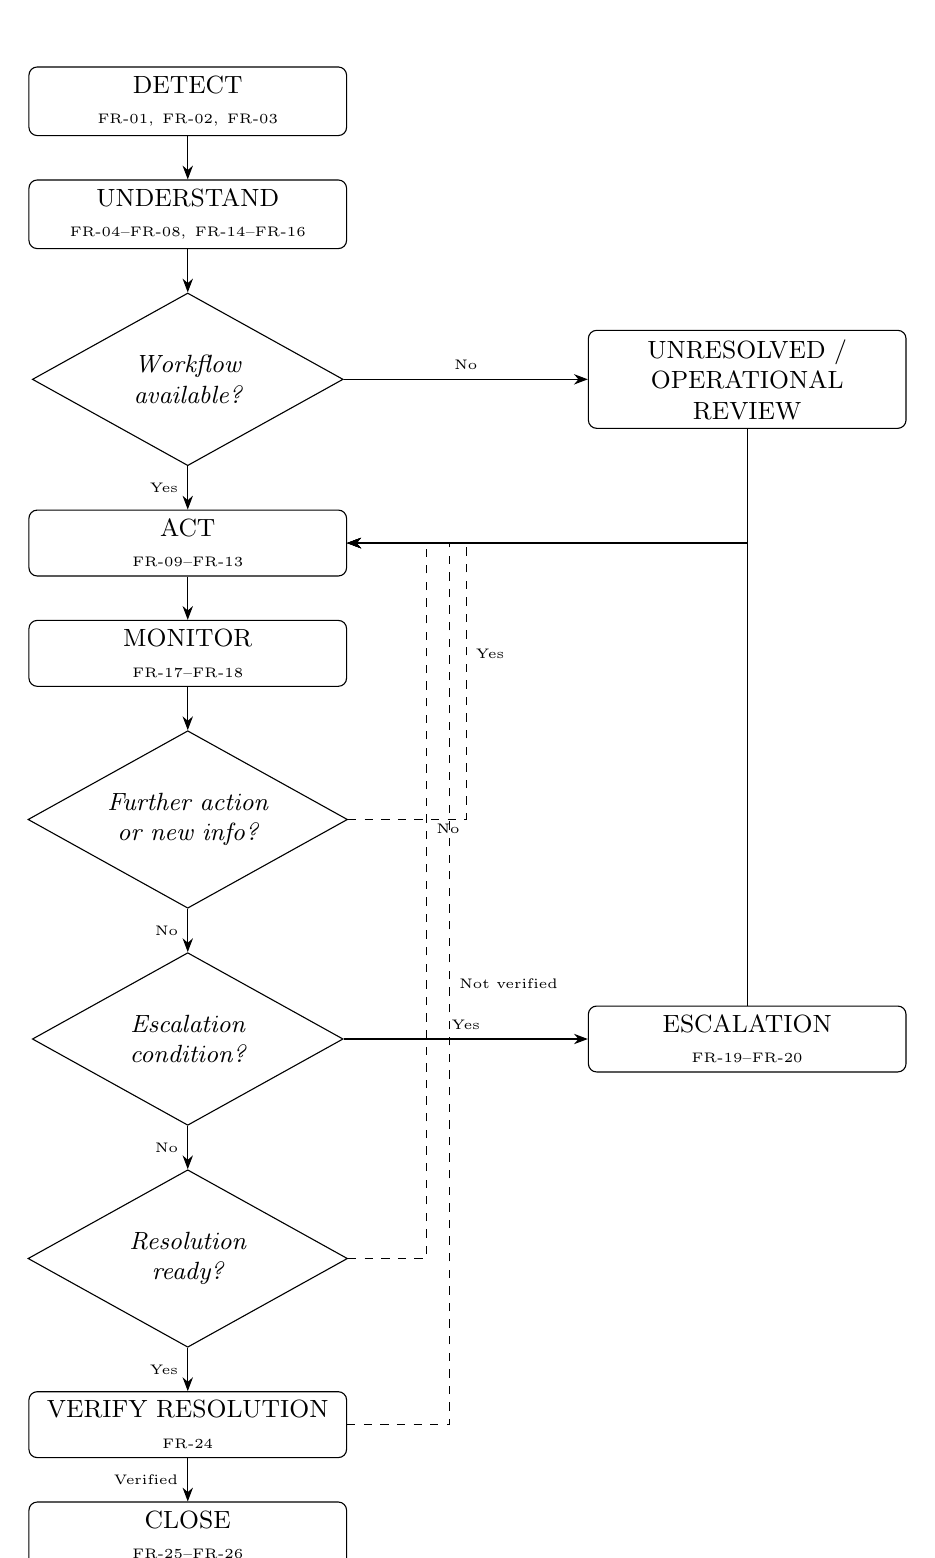
\begin{tikzpicture}[node distance=0.55cm and 2.8cm]

  % Main vertical chain
  \node[state] (detect)  {DETECT\\{\tiny FR-01, FR-02, FR-03}};
  \node[state, below=of detect] (understand) {UNDERSTAND\\{\tiny FR-04–FR-08, FR-14–FR-16}};
  \node[decision, below=of understand] (wf) {Workflow available?};
  \node[state, below=of wf] (act) {ACT\\{\tiny FR-09–FR-13}};
  \node[state, below=of act] (monitor) {MONITOR\\{\tiny FR-17–FR-18}};
  \node[decision, below=of monitor] (event) {Further action or new info?};
  \node[decision, below=of event] (esc) {Escalation condition?};
  \node[decision, below=of esc] (ready) {Resolution ready?};
  \node[state, below=of ready] (verify) {VERIFY RESOLUTION\\{\tiny FR-24}};
  \node[state, below=of verify] (close) {CLOSE\\{\tiny FR-25–FR-26}};

  % Side nodes
  \node[state, right=of wf, xshift=0.3cm] (unresolved) {UNRESOLVED /\\OPERATIONAL REVIEW};
  \node[state, right=of esc, xshift=0.3cm] (escalation) {ESCALATION\\{\tiny FR-19–FR-20}};

  % Main flow arrows
  \draw[arrow] (detect) -- (understand);
  \draw[arrow] (understand) -- (wf);
  \draw[arrow] (wf) -- node[left,font=\tiny]{Yes} (act);
  \draw[arrow] (act) -- (monitor);
  \draw[arrow] (monitor) -- (event);
  \draw[arrow] (event) -- node[left,font=\tiny]{No} (esc);
  \draw[arrow] (esc) -- node[left,font=\tiny]{No} (ready);
  \draw[arrow] (ready) -- node[left,font=\tiny]{Yes} (verify);
  \draw[arrow] (verify) -- node[left,font=\tiny]{Verified} (close);

  % Workflow not available branch
  \draw[arrow] (wf) -- node[above,font=\tiny]{No} (unresolved);
  \draw[arrow] (unresolved) |- (act);

  % Further action
  \draw[darrow] (event.east) -- ++(1.5,0) |- node[right,font=\tiny, pos=0.3]{Yes} (act.east);

  % Escalation branch
  \draw[arrow] (esc) -- node[above,font=\tiny]{Yes} (escalation);
  \draw[arrow] (escalation) |- (act.east);

  % Resolution not ready
  \draw[darrow] (ready.east) -- ++(1.0,0) |- node[right,font=\tiny,pos=0.3]{No} (act.east);

  % Verification failed
  \draw[darrow] (verify.east) -- ++(1.3,0) |- node[right,font=\tiny,pos=0.25]{Not verified} (act.east);

\end{tikzpicture}
\caption{ParcelResolve incident-resolution behavioural model.}
\label{fig:main-model}
\end{figure}

% ============================================================
% SECTION 4 — ALTERNATIVE AND EXCEPTIONAL PATHS
% ============================================================
\section*{4.\enspace Alternative and Exceptional Paths}

A model-based validation should not only check the normal path. The model must also represent behaviour when normal assumptions do not hold.

\begin{figure}[H]
\centering

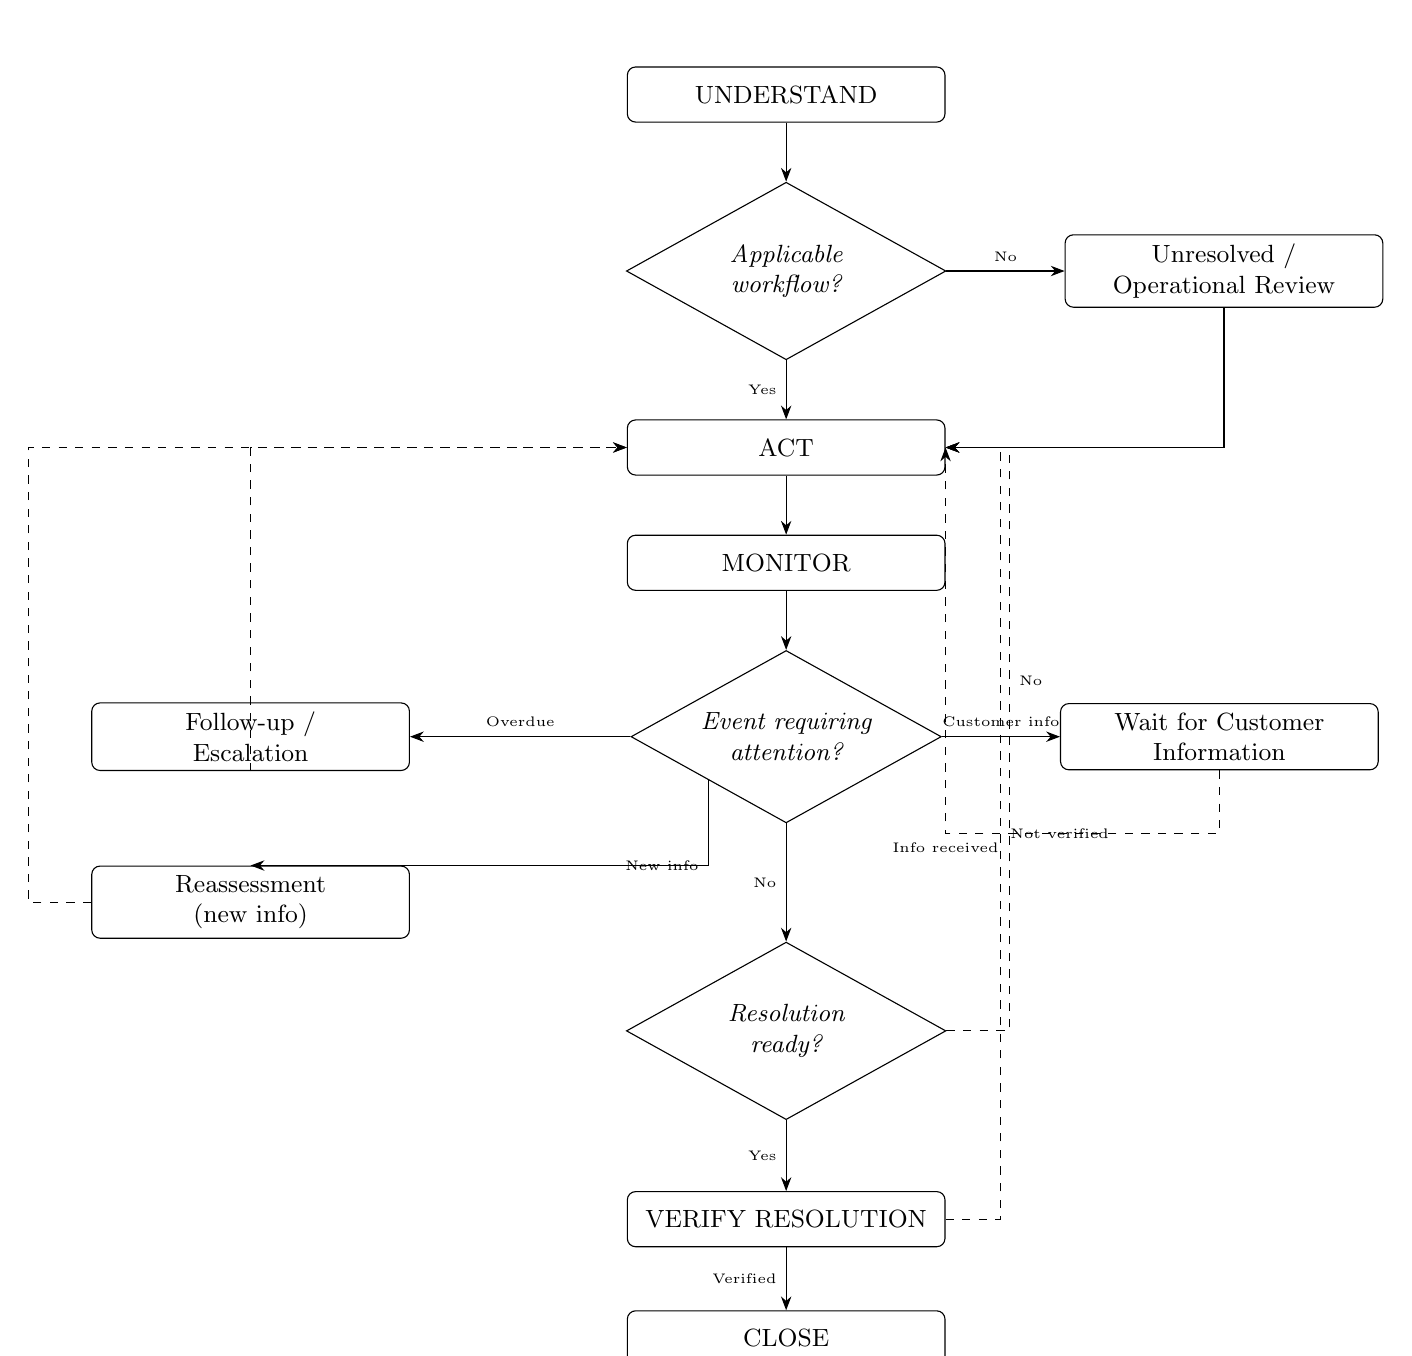
\begin{tikzpicture}[node distance=0.75cm and 1.6cm]

  % =====================================================
  % MAIN FLOW
  % =====================================================

  \node[state] (und) {UNDERSTAND};

  \node[decision, below=of und]
    (awf) {Applicable workflow?};

  \node[state, right=1.5cm of awf]
    (unres) {Unresolved /\\Operational Review};

  \node[state, below=of awf]
    (act) {ACT};

  \node[state, below=of act]
    (mon) {MONITOR};

  \node[decision, below=of mon]
    (evt) {Event requiring\\attention?};

  \node[decision, below=1.5cm of evt]
    (res) {Resolution\\ready?};

  \node[state, below=0.9cm of res]
    (verify) {VERIFY RESOLUTION};

  \node[state, below=0.8cm of verify]
    (close) {CLOSE};


  % =====================================================
  % EXCEPTION PATHS
  % =====================================================

  \node[state, left=2.8cm of evt]
    (fu) {Follow-up /\\Escalation};

  \node[state, below=1.2cm of fu]
    (reassess) {Reassessment\\(new info)};

  \node[state, right=1.5cm of evt]
    (wait) {Wait for Customer\\Information};


  % =====================================================
  % MAIN FLOW
  % =====================================================

  \draw[arrow]
    (und) -- (awf);

  \draw[arrow]
    (awf) -- node[above,font=\tiny]{No} (unres);

  \draw[arrow]
    (awf) -- node[left,font=\tiny]{Yes} (act);

  \draw[arrow]
    (unres) |- (act);

  \draw[arrow]
    (act) -- (mon);

  \draw[arrow]
    (mon) -- (evt);

  \draw[arrow]
    (evt) -- node[left,font=\tiny]{No} (res);

  \draw[arrow]
    (res) -- node[left,font=\tiny]{Yes} (verify);

  \draw[arrow]
    (verify) -- node[left,font=\tiny]{Verified} (close);


  % =====================================================
  % OVERDUE / FOLLOW-UP
  % =====================================================

  \draw[arrow]
    (evt.west) --
    node[above,font=\tiny]{Overdue}
    (fu.east);

  \draw[darrow]
    (fu.south)
    |- (act.west);


  % =====================================================
  % NEW INFORMATION / REASSESSMENT
  % =====================================================

  \draw[arrow]
    (evt.south west)
    |- node[left,font=\tiny]{New info}
    (reassess.north);

  \draw[darrow]
    (reassess.west)
    -- ++(-0.8,0)
    |- (act.west);


  % =====================================================
  % CUSTOMER INFORMATION
  % =====================================================

  \draw[arrow]
    (evt.east) --
    node[above,font=\tiny]{Customer info}
    (wait.west);

  \draw[darrow]
    (wait.south)
    -- ++(0,-0.8)
    -| node[below,font=\tiny]{Info received}
    (act.east);


  % =====================================================
  % RESOLUTION NOT READY
  % =====================================================

  \draw[darrow]
    (res.east)
    -- ++(0.8,0)
    |- node[right,font=\tiny,pos=0.3]{No}
    (act.east);


  % =====================================================
  % VERIFICATION FAILURE
  % =====================================================

  \draw[darrow]
    (verify.east)
    -- ++(0.7,0)
    |- node[right,font=\tiny,pos=0.25]{Not verified}
    (act.east);

\end{tikzpicture}

\caption{Alternative and exceptional behavioural paths.}
\label{fig:alt-paths}
\end{figure}

\subsection*{4.1\enspace No Applicable Workflow}

FR-09 explicitly defines behaviour when no applicable workflow can be selected. The incident enters an unresolved state, an authorised operational user is notified, and the case is forwarded for operational review before proceeding to the Act state. This shows that the requirement has a defined fallback, that an incident cannot become stuck immediately, and that the system does not silently discard an incident.

\subsection*{4.2\enspace Overdue Action}

FR-13 and FR-17 require actions and deadlines to be tracked. When a deadline is exceeded in the Monitor state, a follow-up notification or escalation is triggered, returning the incident to Act or the Escalation path. Overdue actions therefore have an observable consequence in the model, and monitoring is connected to action management and escalation rather than sitting apart from them.

\subsection*{4.3\enspace New Information During Monitoring}

FR-17 requires monitoring for relevant new information. When new information arrives during Monitor, the incident undergoes reassessment and returns to Act. This is one of the reasons we did not model the lifecycle as a strictly one-directional sequence: the process needs to be able to react to changed circumstances.

\subsection*{4.4\enspace Customer Information Required}

Customer communication may require additional information before the incident can progress. Relevant requirements: FR-21 (Customer notification), FR-22 (Additional information request), FR-23 (Communication history). The model represents a waiting condition during Act or Monitor where the incident pauses until the customer provides the necessary information.

\subsection*{4.5\enspace Escalation}

When a configured escalation condition is met during Monitor, the incident transitions to the Escalation state. Escalation may result in reassignment, priority change, notification, or a workflow change before returning to Act or Monitor. Relevant requirements: FR-19 (Escalation), FR-20 (Escalation record).

\subsection*{4.6\enspace Resolution Not Yet Verified}

The model has to distinguish action completion from actual resolution. When resolution conditions are evaluated in Verify~Resolution and found unsatisfied, the incident returns to Act or Monitor, so an incident cannot be closed simply because an operational action was marked complete.

\subsection*{4.7\enspace Successful Resolution}

When resolution conditions are satisfied and verified, the incident transitions from Verify~Resolution to Close, where the closure record is written. Relevant requirements: FR-24, FR-25, FR-26.

% ============================================================
% SECTION 5 — RESTRICTED AND INVALID TRANSITIONS
% ============================================================
\section*{5.\enspace Restricted and Invalid Transitions}

Model-based validation should also identify behaviour that must \textbf{not} be permitted. The following transitions are restricted:

\begin{center}
\small
\texttt{DETECT\;$\rightarrow$\;CLOSE\quad INVALID}\qquad
\texttt{UNDERSTAND\;$\rightarrow$\;CLOSE\quad INVALID}\\[3pt]
\texttt{ACT\;$\rightarrow$\;CLOSE\quad INVALID}\qquad
\texttt{MONITOR\;$\rightarrow$\;CLOSE\quad INVALID}
\end{center}

A valid closure path must include resolution verification: Monitor $\rightarrow$ Verify~Resolution $\rightarrow$ Close.

\begin{figure}[H]
\centering
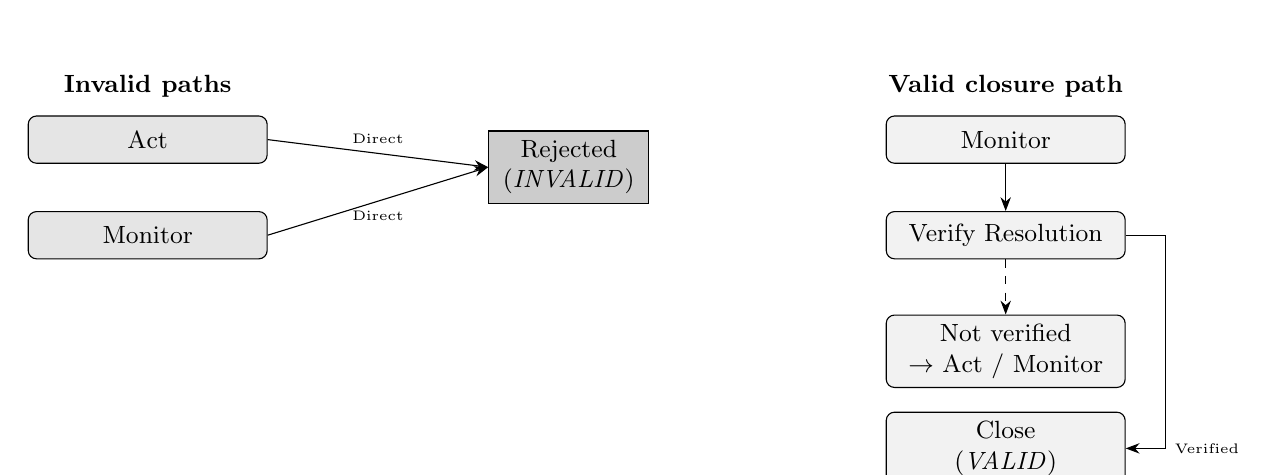
\begin{tikzpicture}[node distance=0.6cm and 1.6cm]

  % Invalid paths column
  \node[invalid] (act) {Act};
  \node[invalid, below=of act] (mon) {Monitor};
  \node[reject, right=of act, xshift=1.2cm, yshift=-0.35cm] (rejected) {Rejected\\\small(\textit{INVALID})};

  \draw[arrow] (act.east) -- node[above,font=\tiny]{Direct} (rejected.west);
  \draw[arrow] (mon.east) -- node[below,font=\tiny]{Direct} (rejected.west);

  % Valid path — separate column
  \node[valid, right=of rejected, xshift=1.4cm, yshift=0.35cm] (mon2) {Monitor};
  \node[valid, below=of mon2] (verify) {Verify Resolution};
  \node[valid, below=of verify, yshift=-0.1cm] (notv) {Not verified\\\small$\rightarrow$ Act / Monitor};
  \node[valid, below=of notv, yshift=0.3cm] (closev) {Close\\\small(\textit{VALID})};

  \draw[arrow] (mon2) -- (verify);
  \draw[darrow] (verify) -- (notv);
  \draw[arrow] (verify.east) -- ++(0.5,0) |- node[right,font=\tiny]{Verified} (closev.east);

  % Labels
  \node[font=\small\bfseries, above=0.1cm of act] {Invalid paths};
  \node[font=\small\bfseries, above=0.1cm of mon2] {Valid closure path};

\end{tikzpicture}
\caption{Valid and invalid closure transitions (supported by FR-24 and FR-25).}
\label{fig:closure}
\end{figure}

This model behaviour is supported by FR-24 and FR-25 and gives us a concrete validation question: \textit{Can an incident be closed without successful resolution verification?} The expected answer is \textbf{no}.

% ============================================================
% SECTION 6 — VALIDATION QUESTIONS
% ============================================================
\section*{6.\enspace Validation Questions}

The following questions are applied to the requirements and behavioural model.

\begin{center}
\small
\begin{tabularx}{\textwidth}{@{} l X l @{}}
\toprule
\textbf{ID} & \textbf{Validation question} & \textbf{Main quality concern} \\
\midrule
VQ-01 & Is the behaviour required by the requirement represented in the model? & Completeness \\
VQ-02 & Is the requirement consistent with the model? & Consistency \\
VQ-03 & Does the model allow behaviour that contradicts the requirement? & Consistency \\
VQ-04 & Are alternative outcomes represented? & Completeness \\
VQ-05 & Are exceptional or failure situations represented? & Completeness \\
VQ-06 & Are transition conditions sufficiently clear? & Clarity / ambiguity \\
VQ-07 & Can the requirement be exercised through a reproducible model scenario? & Testability \\
VQ-08 & Can an incident become stuck without a defined next step? & Completeness \\
VQ-09 & Can a required lifecycle state be bypassed? & Consistency \\
VQ-10 & Does the requirement conflict with another requirement? & Consistency \\
VQ-11 & Does the requirement remain within the product scope? & Scope consistency \\
VQ-12 & Does the behaviour support the stakeholder need identified in Assignment~2? & Traceability \\
VQ-13 & Does the requirement impose an unnecessary implementation choice? & Feasibility / design independence \\
VQ-14 & Can the requirement be validated through a concrete model scenario? & Verifiability \\
\bottomrule
\end{tabularx}
\end{center}

% ============================================================
% SECTION 7 — REQUIREMENT-TO-MODEL MAPPING
% ============================================================
\section*{7.\enspace Requirement-to-Model Mapping}

\subsection*{7.1\enspace Functional Requirements}

\begin{center}
\small
\begin{tabularx}{\textwidth}{@{} l l X @{}}
\toprule
\textbf{Requirement} & \textbf{Model element} & \textbf{Validation focus} \\
\midrule
FR-01 & Detect & System-initiated entry \\
FR-02 & Detect & Customer-initiated entry \\
FR-03 & Detect & Common incident structure \\
FR-04 & Understand & Classification \\
FR-05 & Understand & Information retrieval \\
FR-06 & Understand / lifecycle & Required incident information \\
FR-07 & All lifecycle states & Status progression \\
FR-08 & All lifecycle states & Historical trace \\
FR-09 & Understand $\rightarrow$ Act / Unresolved & Workflow selection and fallback \\
FR-10 & Act & Workflow progression \\
FR-11 & Act & Action creation \\
FR-12 & Act & Responsibility assignment \\
FR-13 & Act / Monitor & Action tracking \\
FR-14 & Understand / Act & Evidence capture \\
FR-15 & Understand / Act & Evidence retrieval \\
FR-16 & Understand / Act & Evidence source/context \\
FR-17 & Monitor & Monitoring conditions \\
FR-18 & Monitor & Follow-up notifications \\
FR-19 & Monitor $\rightarrow$ Escalation & Escalation transition \\
FR-20 & Escalation & Escalation record \\
FR-21 & Act / Monitor & Customer communication \\
FR-22 & Act / Monitor & Additional customer information \\
FR-23 & All relevant states & Communication history \\
FR-24 & Verify Resolution & Resolution verification \\
FR-25 & Verify Resolution $\rightarrow$ Close & Closure condition \\
FR-26 & Close & Closure record \\
FR-27 & Supporting view & Open incident overview \\
FR-28 & Supporting view & Operational resolution information \\
\bottomrule
\end{tabularx}
\end{center}

\subsection*{7.2\enspace Non-Functional Requirements}

Not all NFRs represent states or transitions. They are therefore validated differently.

\begin{center}
\small
\begin{tabularx}{\textwidth}{@{} l X X @{}}
\toprule
\textbf{Requirement} & \textbf{Model relationship} & \textbf{Validation approach} \\
\midrule
NFR-01 & Applies across lifecycle & Check expected performance of model operations \\
NFR-02 & Applies across lifecycle & Check workload/capacity assumptions \\
NFR-03 & Applies across lifecycle & Check availability assumptions \\
NFR-04 & All states & Check preservation of lifecycle data \\
NFR-05 & All states & Check recovery of incident state \\
NFR-06 & Access to model functions & Authentication before protected actions \\
NFR-07 & Access to model functions & Authorisation for state-changing operations \\
NFR-08 & Interfaces & Identify entry points; behaviour itself is not represented in the model \\
NFR-09 & All relevant states & Check handling of personal data \\
NFR-10 & All state changes & Auditability of transitions \\
NFR-11 & Operational interaction & Usability of lifecycle operations \\
NFR-12 & All model elements & Consistent terminology \\
NFR-13 & Workflow behaviour & Configurable rules \\
NFR-14 & Integration transitions & Interface support \\
NFR-15 & Integration transitions & Failure handling \\
NFR-16 & All lifecycle states & Monitoring and observability \\
\bottomrule
\end{tabularx}
\end{center}

% ============================================================
% SECTION 8 — FUNCTIONAL REQUIREMENT VALIDATION
% ============================================================
\section*{8.\enspace Functional Requirement Validation}

\subsection*{8.1\enspace Incident Initiation — FR-01 to FR-03}

\textbf{FR-01 — System-Initiated Incident Creation.} The model represents an external system as an entry point into Detect. An integrated operational system provides information satisfying an incident-detection condition, causing the incident to enter the Detect state. \textit{Result: Consistent with the model.} Validation questions: VQ-01, VQ-06, VQ-07, VQ-12.

\textbf{FR-02 — Customer-Initiated Incident Creation.} A customer or customer-service channel can create an incident and enter the same lifecycle. The customer-initiated path reaches the same Detect/Understand flow as a system-initiated incident. \textit{Result: Consistent.}

\textbf{FR-03 — Incident Standardisation.} Different entry paths converge into a common incident structure before normal processing. The model does not maintain separate resolution lifecycles for the two sources. \textit{Result: Consistent.}

% ============================================================
% SECTION 9
% ============================================================
\section*{9.\enspace Understanding and Assessment — FR-04 to FR-08}

\textbf{FR-04 — Incident Classification.} The model places classification in Understand before workflow selection. The requirement does not claim that classification is always certain, which is appropriate because the classification is based on information available at assessment time. \textit{Result: Consistent.}

\textbf{FR-05 — Incident Information Retrieval.} The model requires relevant information before workflow selection. \textit{Result: Consistent.}

\textbf{FR-06 — Incident Information Management.} The model requires incident information to remain available throughout the lifecycle. \textit{Result: Consistent.}

\textbf{FR-07 — Incident Status Management.} The model changes lifecycle state as the incident progresses, providing a clear basis for status management. \textit{Result: Consistent.}

\textbf{FR-08 — Incident History.} The model contains multiple state transitions and activities, providing a clear basis for maintaining chronological history. \textit{Result: Consistent.}

% ============================================================
% SECTION 10
% ============================================================
\section*{10.\enspace Workflow and Action Management — FR-09 to FR-13}

\textbf{FR-09 — Workflow Selection.} The model explicitly represents two paths: (1)~applicable workflow found; (2)~no applicable workflow found. The second path enters an unresolved state and requires operational review. \textit{Result: Consistent and important for completeness.}

\textbf{FR-10 — Workflow Progression.} The model tracks movement through Act and Monitor and allows the process to return to Act when further action is required. \textit{Result: Consistent.}

\textbf{FR-11 — Action Creation.} Actions are created in the Act state. \textit{Result: Consistent.}

\textbf{FR-12 — Action Assignment.} The Act state includes assignment to a responsible operational role or user. \textit{Result: Consistent.}

\textbf{FR-13 — Action Tracking.} The model connects action tracking with Monitor, where deadlines and overdue conditions are evaluated. \textit{Result: Consistent.}

% ============================================================
% SECTION 11
% ============================================================
\section*{11.\enspace Evidence — FR-14 to FR-16}

Evidence is represented primarily within Understand and Act. The model supports recording and reference of evidence; retrieval of evidence; and source and context information. The model does not require ParcelResolve to become the primary storage system for external evidence.

\textit{Validation result: FR-14, FR-15, and FR-16 are consistent with the model.}

% ============================================================
% SECTION 12
% ============================================================
\section*{12.\enspace Monitoring and Escalation — FR-17 to FR-20}

\textbf{FR-17 — Incident Monitoring.} Monitor is explicitly defined as a state in which open incidents and actions are checked for configured conditions. \textit{Result: Consistent.}

\textbf{FR-18 — Follow-Up Notification.} The model permits monitoring conditions to generate a follow-up notification. \textit{Result: Consistent.}

\textbf{FR-19 — Escalation.} The model includes Escalation as an alternative path from Monitor. \textit{Result: Consistent.}

\textbf{FR-20 — Escalation Record.} The model allows escalation information to be recorded before returning to operational handling. \textit{Result: Consistent.}

% ============================================================
% SECTION 13
% ============================================================
\section*{13.\enspace Customer Communication — FR-21 to FR-23}

Customer communication is treated as supporting behaviour that may occur during Act and Monitor. The model supports communicating incident status, requesting additional information, and recording communication history.

\textbf{Validation point.} FR-22 introduces a possible waiting condition when additional customer information is required. A refined model should therefore represent this explicitly rather than assuming that every incident can continuously progress without waiting for external information.

\textit{Current result: No contradiction identified. The waiting condition should be made explicit in the detailed model.}

% ============================================================
% SECTION 14
% ============================================================
\section*{14.\enspace Resolution Verification and Closure — FR-24 to FR-26}

This is a critical part of the model.

\textbf{FR-24 — Resolution Verification.} The model contains a dedicated Verify~Resolution state. \textit{Result: Consistent.}

\textbf{FR-25 — Incident Closure.} The model allows Close only after successful verification. \textit{Result: Consistent.}

\textbf{FR-26 — Closure Record.} The Close state records the resolution outcome, closure time, and relevant supporting information. \textit{Result: Consistent.}

\textbf{Critical validation rule.} The model must reject \texttt{Act $\rightarrow$ Close} and \texttt{Monitor $\rightarrow$ Close}, and require \texttt{Monitor $\rightarrow$ Verify Resolution $\rightarrow$ Close}. This provides a concrete model-based validation of FR-24 and FR-25.

% ============================================================
% SECTION 15
% ============================================================
\section*{15.\enspace Operational Insights — FR-27 to FR-28}

FR-27 and FR-28 are supporting operational capabilities rather than lifecycle transitions. The model provides the incident states, actions, deadlines, escalation information, and resolution outcomes that these operational views depend on. FR-28's filtering dimensions — incident type, date, responsible team, and escalation state — are represented as incident attributes or lifecycle information within the model.

\textit{Validation result: Consistent.}

% ============================================================
% SECTION 16 — NFR VALIDATION
% ============================================================
\section*{16.\enspace Non-Functional Requirement Validation}

The behavioural model cannot fully validate every quality attribute. NFRs therefore receive one of three validation treatments: (1)~\textbf{Model-validatable} — the model directly represents the requirement's behaviour; (2)~\textbf{Partially model-validatable} — the model provides conditions or interactions to validate, but additional testing is needed; (3)~\textbf{Not fully model-validatable} — the model can expose relevant dependencies, but quantitative or implementation-level validation requires additional techniques.

\subsection*{16.1\enspace Performance and Capacity}

\textbf{NFR-01.} The model identifies operations and transitions that need to occur during incident processing. Model contribution: identifies where response-time expectations apply. Additional validation required: performance testing using defined workload and response-time thresholds. \textit{Result: Partially model-validatable.}

\textbf{NFR-02.} The model represents the number and types of operational activities, users, and integration events. Additional validation required: capacity/load testing. \textit{Result: Partially model-validatable.}

\subsection*{16.2\enspace Availability and Reliability}

\textbf{NFR-03.} Availability is a system-wide quality property rather than a transition. \textit{Result: Not fully model-validatable.}

\textbf{NFR-04.} The model can identify information that must survive transitions and failures. \textit{Result: Partially model-validatable.}

\textbf{NFR-05.} The model can define the expected incident state after recovery. \textit{Result: Partially model-validatable.}

\subsection*{16.3\enspace Security and Access Control}

\textbf{NFR-06.} The model can require authentication before protected operations. \textit{Result: Partially model-validatable.}

\textbf{NFR-07.} The model can represent which roles may perform protected lifecycle operations. \textit{Result: Partially model-validatable.}

\textbf{NFR-08.} \textit{(Reclassified after Claude review — see Section~C, decision C-07.)} The model identifies where external interfaces sit in the lifecycle, but request-rate behaviour itself is not represented as a state, transition, or condition anywhere in the model — the model gives us a location to test against, not a mechanism to validate. \textit{Result: Not fully model-validatable.}

\textbf{NFR-09.} The model identifies states where personal information may be processed. Full validation requires security/privacy analysis and implementation-level verification. \textit{Result: Partially model-validatable.}

\subsection*{16.4\enspace Auditability}

\textbf{NFR-10.} The model contains state changes and activities that should produce auditable records. \textit{Result: Partially model-validatable.}

\subsection*{16.5\enspace Usability and Consistency}

\textbf{NFR-11.} The model can identify the actions users must perform, but usability itself requires user evaluation or usability testing. \textit{Result: Not fully model-validatable.}

\textbf{NFR-12.} The model provides a controlled set of states and concepts to support validation of terminology consistency. \textit{Result: Model can support validation of terminology consistency.}

\subsection*{16.6\enspace Maintainability and Integration}

\textbf{NFR-13.} The model identifies workflow selection as a rule-dependent transition. \textit{Result: Partially model-validatable.}

\textbf{NFR-14.} The model explicitly includes external systems as entry and information sources. \textit{Result: Partially model-validatable.}

\textbf{NFR-15.} The model should include an integration-failure path so that an unavailable external system does not leave an incident without a defined state. The requirement is relevant to the model, but the failure transition should be represented explicitly in the detailed model (and in the diagrams themselves — see Section~C, decision C-10). \textit{Result: Relevant to the model; explicit failure path to be added.}

\subsection*{16.7\enspace Observability}

\textbf{NFR-16.} The model identifies lifecycle transitions, monitoring conditions, and escalation events that require operational visibility. \textit{Result: Partially model-validatable.}

% ============================================================
% SECTION 17 — SCENARIO-BASED MODEL VALIDATION
% ============================================================
\section*{17.\enspace Scenario-Based Model Validation}

The following scenarios are used to exercise the model.

\begin{center}
\small
\begin{tabularx}{\textwidth}{@{} l X X @{}}
\toprule
\textbf{Scenario} & \textbf{Expected path} & \textbf{Main requirements} \\
\midrule
S-01 Normal system incident & Detect → Understand → Act → Monitor → Verify → Close & FR-01, FR-04, FR-09, FR-24, FR-25 \\
S-02 Customer incident & Customer entry → Detect → Understand → Act → Monitor & FR-02, FR-03 \\
S-03 No workflow & Understand → Unresolved → Operational Review → Act & FR-09 \\
S-04 Overdue action & Act → Monitor → Overdue → Follow-up / Escalation & FR-13, FR-17, FR-18, FR-19 \\
S-05 New information & Monitor → New information → Act → Monitor & FR-17 \\
S-06 Customer information required & Act/Monitor → Request information → Wait → Resume & FR-21, FR-22, FR-23 \\
S-07 Escalation & Monitor → Escalation → Act / Monitor & FR-19, FR-20 \\
S-08 Resolution not verified & Monitor → Verify → Failed → Act / Monitor & FR-24 \\
S-09 Successful resolution & Monitor → Verify → Close & FR-24, FR-25, FR-26 \\
S-10 Invalid closure attempt & Act/Monitor → Close & Must be rejected \\
S-11 Integration failure & External interaction → Failure handling → Recover / Review & FR-05, NFR-14, NFR-15 \\
S-12 Protected operation & Unauthenticated request → Denied → Authentication → Operation & NFR-06, NFR-07 \\
\bottomrule
\end{tabularx}
\end{center}

\textit{Two further scenarios were proposed during the Claude review (S-13, S-14) to cover the permanently-unmatched-workflow and repeated-escalation cases identified in Section~C. They are not yet added to the model diagrams; see decisions C-03 and C-06.}

% ============================================================
% SECTION 18 — VALIDATION RESULTS SUMMARY
% ============================================================
\section*{18.\enspace Validation Results Summary}

The current model provides coverage for all \textbf{28 functional requirements}.

\begin{center}
\small
\begin{tabularx}{\textwidth}{@{} l r X @{}}
\toprule
\textbf{Area} & \textbf{Requirements} & \textbf{Model result} \\
\midrule
Incident initiation        & FR-01–FR-03 & Covered \\
Assessment and information & FR-04–FR-08 & Covered \\
Workflow and actions       & FR-09–FR-13 & Covered \\
Evidence                   & FR-14–FR-16 & Covered \\
Monitoring and escalation  & FR-17–FR-20 & Covered \\
Customer communication     & FR-21–FR-23 & Covered, with waiting behaviour to refine \\
Resolution and closure     & FR-24–FR-26 & Covered \\
Operational insights       & FR-27–FR-28 & Covered \\
\bottomrule
\end{tabularx}
\end{center}

All \textbf{16 non-functional requirements} are reviewed, but they are not all directly expressible as state transitions.

\begin{center}
\small
\begin{tabularx}{\textwidth}{@{} X l @{}}
\toprule
\textbf{NFR validation category} & \textbf{Requirements} \\
\midrule
Directly / partially supported by model & NFR-04, NFR-06, NFR-07, NFR-10, NFR-12, NFR-13, NFR-14, NFR-15, NFR-16 \\
Partially supported; requires additional testing & NFR-01, NFR-02, NFR-05, NFR-09 \\
Requires additional validation technique & NFR-03, NFR-08, NFR-11 \\
\bottomrule
\end{tabularx}
\end{center}

\textit{NFR-08 was moved from the middle row to the bottom row after the Claude review (decision C-07 in Section~C); it was originally listed under "partially supported."}

This distinction is important because Model-Based Validation should not be presented as sufficient evidence for every type of non-functional requirement.

% ============================================================
% SECTION 19 — ISSUES AND REFINEMENTS
% ============================================================
\section*{19.\enspace Issues and Refinements Identified}

\subsection*{19.1\enspace Explicit Waiting State for Customer Information}

\textbf{Requirement: FR-22.} The model should explicitly represent a waiting condition when an incident cannot progress until additional customer information is received. Without an explicit waiting condition, the model may imply that the incident can immediately continue processing. Proposed refinement: add a \texttt{Waiting for Customer Information} state. The current FR-22 requirement can remain unless later analysis shows that the waiting behaviour itself needs to be stated more precisely.

\subsection*{19.2\enspace Explicit Closure Restriction}

\textbf{Requirements: FR-24 and FR-25.} The model demonstrates that closure must not be reachable directly from Act or Monitor. Decision: preserve the existing requirements and make the restriction explicit in the behavioural model.

\subsection*{19.3\enspace Explicit Integration Failure Path}

\textbf{Requirement: NFR-15.} The model should represent what happens when an integrated system is unavailable or returns an unusable response. Decision: add an integration-failure path to the detailed model, and reflect it in the diagrams in Figures~1 and~2, not only in this narrative section (see Section~C, decision C-10). The exact recovery mechanism should remain outside the requirements model unless specified later.

\subsection*{19.4\enspace Quantitative NFR Thresholds}

\textbf{Requirements: NFR-01, NFR-02, NFR-03, NFR-05, NFR-08.} The current requirements intentionally avoid arbitrary numerical values because Assignment~2 did not establish sufficient operational baselines. Decision: do not invent thresholds during model validation. These values should be established later using operational data, stakeholder agreement, or system constraints.

\subsection*{19.5\enspace No Terminal Outcome for a Permanently Unmatched Workflow}

\textbf{Requirement: FR-09.} \textit{(Raised during Claude review, accepted — see Section~C, decision C-03.)} FR-09 defines a fallback when no workflow can be matched at classification time (Unresolved / Operational Review), and Figure~1 sends that path back into Act. Neither the requirement nor the current model says what happens if operational review still cannot resolve the incident into a workflow — the model has no terminal outcome for this case, so an incident could in principle loop between Unresolved and Act indefinitely. Proposed refinement for the detailed model: add an outcome such as manual resolution or referral to management for incidents that operational review cannot place into a workflow after a defined number of attempts. We are not changing FR-09 itself, since the exact escalation path for this case needs input from the host organisation; the gap is noted here for the next revision.

\subsection*{19.6\enspace No Bound on Repeated Escalation}

\textbf{Requirements: FR-19, FR-20.} \textit{(Raised during Claude review, accepted — see Section~C, decision C-06.)} The Escalation path (Monitor $\rightarrow$ Escalation $\rightarrow$ Act/Monitor) can repeat without limit in the current model; nothing represents a maximum escalation count or a terminal "requires manual intervention" outcome if repeated escalation keeps failing to resolve the incident. This is a completeness gap in the model rather than a defect in FR-19/FR-20 as written. Proposed refinement for the detailed model: track escalation count per incident and define a terminal outcome once a configured limit is reached.

% ============================================================
% SECTION 20
% ============================================================
\section*{20.\enspace Requirements That Are Not Fully Validated by the Behavioural Model}

Model-Based Validation is useful but has limits. The following aspects require additional validation techniques: exact performance measurements; capacity limits; availability percentages; recovery time and recovery point targets; usability with real operational users; security penetration testing; privacy compliance verification; actual integration reliability; and implementation-level observability.

Therefore, a requirement being compatible with the behavioural model does \textbf{not} mean that the implemented system has been proven to satisfy it. The model validates the coherence and expected behaviour represented by the requirement.

Two further points came up during the Claude review and are tracked as open points rather than resolved here, in the same spirit as the open points list in Assignment~3, Section~D.8: incident cancellation/withdrawal is not addressed by any current FR (see Section~C, decision C-04), and duplicate-incident handling when the same parcel problem is reported through more than one channel is not addressed by FR-01–FR-03 (see Section~C, decision C-05). Neither is treated as a defect in the current requirements, since Assignment~2 did not establish whether either case is in scope — they are flagged for a future requirements pass.

% ============================================================
% SECTION 21
% ============================================================
\section*{21.\enspace Human Judgment and Model Contribution}

The behavioural model gives us a systematic way to look for missing transitions, unreachable states, invalid transitions, missing alternative paths, missing exception paths, lifecycle inconsistencies, and requirements that cannot be exercised through a clear scenario.

However, the model itself does not decide whether a requirement is appropriate for the organisation. Human judgment is still required to determine: whether the model represents the intended business process; whether a requirement is sufficiently precise; whether a proposed refinement changes the intended scope; whether a quality target is realistic; and whether stakeholder needs are correctly represented.

The model is a validation aid, not a replacement for requirements engineering judgment.

% ============================================================
% SECTION 22
% ============================================================
\section*{22.\enspace Limitations of the Validation}

This validation has several limitations.

\begin{enumerate}
  \item The behavioural model is derived from the requirements and product lifecycle, so an incorrect assumption in the source requirements can also appear in the model.
  \item Quantitative non-functional requirements cannot be proven through a state-transition model alone.
  \item Some operational details, such as exact escalation rules and integration failure recovery, are not yet specified.
  \item The model does not represent the internal software architecture or implementation technology.
  \item Stakeholder acceptance and usability require validation with real users.
  \item The current model is a requirements-level behavioural model, not an executable model-based testing environment.
  \item The Claude review in Section~C is a second opinion, not an independent validation technique — it was applied to the same requirements and the same model, so it cannot catch a gap in the underlying lifecycle assumption from Assignment~2 itself.
\end{enumerate}

% ============================================================
% SECTION 23 — CONCLUSION
% ============================================================
\section*{23.\enspace Conclusion}

The Model-Based Validation shows that the ParcelResolve requirements describe a coherent incident-resolution lifecycle from detection through verified closure. The main lifecycle is:

\begin{center}
\textbf{Detect $\rightarrow$ Understand $\rightarrow$ Act $\rightarrow$ Monitor $\rightarrow$ Verify Resolution $\rightarrow$ Close}
\end{center}

The model also represents important alternative and exceptional paths, including system-initiated and customer-initiated incidents; absence of an applicable workflow; overdue actions; escalation; new information; customer information requests; unsuccessful resolution verification; and integration and access-control conditions.

No major contradiction between the functional requirements and the current lifecycle model has been identified. The main refinements identified are the explicit representation of waiting for customer information, integration failure handling, the restriction that closure must follow successful resolution verification, and — after the Claude review — a terminal outcome for permanently unmatched workflows and a bound on repeated escalation.

The validation also demonstrates that Model-Based Validation is more directly applicable to behavioural functional requirements than to quantitative or experiential non-functional requirements. Additional validation techniques will therefore be required for performance, availability, usability, security, privacy, and other implementation-level quality concerns.

\vspace{6pt}\hrule\vspace{8pt}

% ============================================================
% ASSIGNMENT 4 — A/B/C STRUCTURE
% ============================================================
{\centering\large\bfseries Assignment 4 — Requirements Review Process and Results\par}
\vspace{6pt}

This section presents the Assignment~4 submission structure separately from the Model-Based Validation report above.

% ============================================================
% SECTION A — REQUIREMENTS REVIEW PROCESS
% ============================================================
\section*{A.\enspace Requirements Review Process}

\subsection*{A.1\enspace Self Analysis}

\subsubsection*{Technique}

We selected \textbf{Model-Based Validation (MBV)} as the requirements review technique. ParcelResolve has a defined incident-resolution lifecycle and many of its requirements describe behavioural changes, transitions, conditions, and alternative paths, so a behavioural model gives us a way to review the requirements as a connected process rather than as isolated statements.

\subsubsection*{Inputs and Scope}

The main input was the Requirements Specification prepared in Assignment~3. The review covers FR-01–FR-28, NFR-01–NFR-16, and 44 requirements in total. The product vision, scope, stakeholder analysis, and lifecycle from Assignment~2 were used as context.

\subsubsection*{Behavioural Model}

The main lifecycle used for validation is:

\begin{center}
\textbf{Detect $\rightarrow$ Understand $\rightarrow$ Act $\rightarrow$ Monitor $\rightarrow$ Verify Resolution $\rightarrow$ Close}
\end{center}

The model also includes alternative and exceptional behaviour: no applicable workflow; unresolved state and operational review; overdue actions; escalation; new information; waiting for customer information; unsuccessful resolution verification; integration failure; and authentication and authorisation conditions.

The model is a requirements-level behavioural model. It is not an implementation or software architecture model.

\subsubsection*{Validation Process}

The requirements were mapped to states, transitions, conditions, or supporting behaviour in the model. The validation then considered normal, alternative, exceptional, and invalid scenarios, applying the 14 validation questions listed in Section~6.

\subsubsection*{Scenarios Used}

The main scenarios considered were: normal system-initiated incident; customer-initiated incident; no applicable workflow; overdue action; new information during monitoring; additional customer information required; escalation; resolution not yet verified; successful resolution; invalid closure attempt; integration failure; and authentication/authorisation failure.

\subsubsection*{Treatment of NFRs}

The behavioural model does not fully validate every type of NFR. Some NFRs can be related to model behaviour, while others require additional techniques such as performance testing, capacity testing, usability evaluation, security testing, privacy analysis, or availability testing. We used the model to identify where NFRs apply, without treating model compatibility as proof that an NFR is satisfied by an implementation.

\subsubsection*{Evidence and Reproducibility}

The validation can be reproduced using: the Assignment~3 requirements; the behavioural model; the requirement-to-model mapping; the validation questions; the validation scenarios; and the documented findings and decisions. No automated model-checking tool was used.

\vspace{8pt}
\subsection*{A.2\enspace Review with Claude}

We asked Claude to review the Model-Based Validation process in A.1 against the Assignment~3 requirements specification, looking for missing states or transitions, overlooked alternative or exceptional paths, unclear validation questions, weaknesses in traceability, gaps in the treatment of NFRs, and anything that would affect reproducibility. The points below are Claude's observations. Each is marked \textbf{[SELF]} where it confirms something already in our own analysis, or \textbf{[AI PROPOSAL]} where it is a new point raised during this review.

\begin{itemize}
  \item \textbf{[SELF]} The waiting condition for customer information (FR-22, Section~19.1) and the missing integration-failure path (NFR-15, Section~19.3) were already identified as gaps in our self-analysis. Claude's review agreed with both and did not suggest changing the proposed refinements.
  \item \textbf{[AI PROPOSAL]} The model does not show what happens if an incident permanently fails to match a resolution workflow. Figure~1 sends the \texttt{UNRESOLVED / OPERATIONAL REVIEW} state back into \texttt{ACT}, but there is no outcome for the case where operational review still cannot find an applicable workflow after that.
  \item \textbf{[AI PROPOSAL]} Neither the requirements nor the model address incident cancellation or withdrawal — for example the customer withdraws the report, or the incident turns out to be a duplicate or an invalid report. FR-24–FR-26 assume every incident is eventually resolved and verified; there is no closure path that does not go through Verify~Resolution.
  \item \textbf{[AI PROPOSAL]} FR-03 (Incident Standardisation) converts incidents from different sources into a common structure, but does not address the case where the same underlying parcel problem produces two separate incidents — for example detected automatically by an integrated system and also reported by the customer for the same parcel.
  \item \textbf{[AI PROPOSAL]} The escalation path (Monitor $\rightarrow$ Escalation $\rightarrow$ Act/Monitor) can, in the current model, repeat indefinitely. There is no maximum escalation count or terminal outcome represented for an incident that keeps failing to resolve after repeated escalation.
  \item \textbf{[AI PROPOSAL]} FR-07 refers to "the current status" of an incident, but the specification does not enumerate status values or map them onto the lifecycle state names used in the model (Detect, Understand, Act, Monitor, Escalation, Verify Resolution, Close). An explicit mapping would strengthen traceability between FR-07 and the model.
  \item \textbf{[AI PROPOSAL]} Several requirements use qualifiers such as "relevant," "sufficient," and "appropriate" without further definition (e.g. FR-05, FR-06, FR-16, NFR-04, NFR-09). This is consistent with our own approach in Assignment~3 (Section~D.8) of deferring precise operational detail, but it does mean some of these requirements cannot be exercised through a single, unambiguous model scenario yet.
\end{itemize}

These are proposals, not automatic changes. Section~C records which ones we accepted, deferred, or rejected, and why.

% ============================================================
% SECTION B — VALIDATION RESULTS
% ============================================================
\section*{B.\enspace Validation Results}

\subsection*{B.1\enspace Self Analysis}

\subsubsection*{Requirements Reviewed}

A total of \textbf{44 requirements} were reviewed: 28 functional requirements (FR-01–FR-28) and 16 non-functional requirements (NFR-01–NFR-16).

\subsubsection*{Functional Requirement Results}

\begin{center}
\small
\begin{tabularx}{\textwidth}{@{} l r X @{}}
\toprule
\textbf{Requirement area} & \textbf{Requirements} & \textbf{Self-analysis result} \\
\midrule
Incident initiation        & FR-01–FR-03 & Covered \\
Assessment and information & FR-04–FR-08 & Covered \\
Workflow and actions       & FR-09–FR-13 & Covered \\
Evidence                   & FR-14–FR-16 & Covered \\
Monitoring and escalation  & FR-17–FR-20 & Covered \\
Customer communication     & FR-21–FR-23 & Covered, with waiting behaviour to refine \\
Resolution and closure     & FR-24–FR-26 & Covered \\
Operational insights       & FR-27–FR-28 & Covered \\
\bottomrule
\end{tabularx}
\end{center}

\subsubsection*{Main Findings}

The self-analysis did not identify a major contradiction between the functional requirements and the main incident-resolution lifecycle. The following points were identified for refinement.

\textbf{FR-22 — Customer information waiting.} The model should explicitly represent a waiting condition when additional customer information is required. The proposed path is: Act / Monitor $\rightarrow$ Customer information required $\rightarrow$ Waiting for Customer Information $\rightarrow$ Information received $\rightarrow$ Understand / Act.

\textbf{FR-24 / FR-25 — Resolution verification before closure.} The model must prevent an incident from being closed directly from Act or Monitor. The valid closure path is: Monitor $\rightarrow$ Verify Resolution $\rightarrow$ Verified $\rightarrow$ Close; or Monitor $\rightarrow$ Verify Resolution $\rightarrow$ Not verified $\rightarrow$ Act / Monitor. Direct transitions Act $\rightarrow$ Close and Monitor $\rightarrow$ Close are invalid.

\textbf{NFR-15 — Integration failure.} The model should explicitly represent what happens when an external integration is unavailable or returns an unusable response.

\textbf{NFR-01, NFR-02, NFR-03, NFR-05, and NFR-08.} The current requirements do not contain justified numerical thresholds. These should not be invented during validation and should be defined later using appropriate operational evidence and stakeholder agreement.

\textbf{NFR-11 — Usability.} Usability cannot be fully validated through the behavioural model. Additional user-oriented validation is required.

\subsubsection*{NFR Results}

\begin{center}
\small
\begin{tabularx}{\textwidth}{@{} X l X @{}}
\toprule
\textbf{Validation category} & \textbf{Requirements} & \textbf{Self-analysis result} \\
\midrule
Directly or partially supported by the model & NFR-04, NFR-06, NFR-07, NFR-10, NFR-12, NFR-13, NFR-14, NFR-15, NFR-16 & Model provides useful validation \\
Partially supported, requiring additional testing & NFR-01, NFR-02, NFR-05, NFR-08, NFR-09 & Additional validation required \\
Not fully model-validatable & NFR-03, NFR-11 & Additional validation technique required \\
\bottomrule
\end{tabularx}
\end{center}

\textit{Note: NFR-08 was moved into the "Not fully model-validatable" row after the Claude review (see B.2 and Section~C, decision C-07); this table reflects the original self-analysis classification, and Section~18 shows the revised version.}

\subsubsection*{Overall Self-Analysis Result}

The behavioural model represents the main ParcelResolve lifecycle and provides coverage for all 28 functional requirements. The main refinement areas are: (1)~waiting for customer information; (2)~preventing closure before successful resolution verification; (3)~integration failure handling; (4)~later definition of quantitative NFR targets; and (5)~additional validation techniques for NFRs that cannot be fully evaluated through the behavioural model.

\vspace{8pt}
\subsection*{B.2\enspace Review with Claude}

We asked Claude to check whether any requirement was incorrectly classified as covered, whether an important scenario is missing, whether any finding should be classified differently, whether any NFR was treated too strongly or too weakly, and whether any conclusion in B.1 is unsupported by the model.

\begin{itemize}
  \item \textbf{[SELF]} The self-analysis correctly identifies FR-22, FR-24/FR-25, and NFR-15 as the main areas needing refinement. Claude's review did not find these classifications incorrect.
  \item \textbf{[AI PROPOSAL]} NFR-08 (protection against excessive requests) was listed as "partially supported; requires additional testing." On review, the model does not actually give NFR-08 behavioural coverage beyond identifying that interfaces exist — request-rate behaviour is not represented as a state, transition, or condition anywhere in the model. Claude recommends reclassifying NFR-08 as \textit{not fully model-validatable}, alongside NFR-03 and NFR-11.
  \item \textbf{[AI PROPOSAL]} The functional coverage claims (FR-01–FR-28 "Covered" in Sections~8–15 and the B.1 table) are consistent with the requirement-to-model mapping in Section~7 and the scenario list in Section~17. Claude did not find a functional requirement that was incorrectly marked as covered.
  \item \textbf{[AI PROPOSAL]} The scenario table in Section~17 has no scenario for the permanently-unmatched-workflow case or for repeated escalation (see A.2). Adding scenarios for these would make the edge cases explicit and testable, in line with VQ-07 and VQ-08.
  \item \textbf{[AI PROPOSAL]} The self-analysis states that no major contradiction was found between the functional requirements and the lifecycle. Claude's review agrees: no requirement was found to require a transition the model marks invalid (Section~5), and no invalid transition was found to be implied by a requirement.
\end{itemize}

Section~C records the group's decisions on these points.

% ============================================================
% SECTION C — REVIEW DECISION RECORD
% ============================================================
\section*{C.\enspace Review Decision Record}

After the Claude review, accepted suggestions are recorded here rather than silently merged into the self-analysis. This makes it possible to distinguish the group's own analysis from AI-supported suggestions and demonstrates that final decisions were made by the group.

\begin{center}
\small
\begin{tabularx}{\textwidth}{@{} l l X >{\centering\arraybackslash}p{1.9cm} X @{}}
\toprule
\textbf{ID} & \textbf{Source} & \textbf{Proposal} & \textbf{Decision} & \textbf{Reason} \\
\midrule
C-01 & Self Analysis & Add explicit \texttt{Waiting for Customer Information} state for FR-22. & Accepted & Prevents the model from implying an incident can always progress without external input; already reflected in Section~19.1. \\
C-02 & Self Analysis & Add explicit integration-failure path for NFR-15. & Accepted & Prevents an unavailable external system from leaving an incident in an undefined state; already reflected in Section~19.3. \\
C-03 & Claude Review & Add a terminal outcome for incidents that permanently fail to match a workflow (FR-09). & Accepted (Modify) & Real completeness gap — the current model allows an unresolved incident to loop indefinitely. Recorded as Section~19.5; exact escalation mechanism deferred to a later revision with host-organisation input. \\
C-04 & Claude Review & Add incident cancellation / withdrawal handling. & Deferred & Not addressed anywhere in the Assignment~2 scope; we cannot tell whether it is in scope without asking the host organisation. Logged as an open point in Section~20. \\
C-05 & Claude Review & Add duplicate-incident detection across FR-01/FR-02. & Deferred & Same reasoning as C-04 — plausible real-world gap, but not something Assignment~2 tells us is in scope. Logged as an open point in Section~20. \\
C-06 & Claude Review & Add a bound on repeated escalation (FR-19/FR-20). & Accepted (Modify) & Same category of gap as C-03: the model doesn't currently stop an incident cycling through escalation forever. Recorded as Section~19.6. \\
C-07 & Claude Review & Reclassify NFR-08 from "partially model-validatable" to "not fully model-validatable." & Accepted & On inspection the model gives no actual behavioural coverage of rate-limiting; the original classification overstated what the model checks. Applied to Sections~16.3, 18, and noted in B.1. \\
C-08 & Claude Review & Flag ambiguous qualifiers ("relevant," "sufficient," "appropriate") across several FRs/NFRs. & Noted, not changed & Consistent with our own decision in Assignment~3 (D.8) to defer precise operational detail until a baseline exists; re-wording now would risk inventing detail we don't have. Logged as a limitation. \\
C-09 & Claude Review & Map FR-07 status values explicitly onto model state names. & Deferred & Useful for a detailed design-level model, not essential for requirements-level validation at this stage. \\
C-10 & Claude Review & Reflect the NFR-15 integration-failure path in Figures~1 and~2, not just in the narrative text. & Accepted & Paired with C-02; the diagrams should match what the text already claims. To be applied when the detailed model diagrams are next revised. \\
\bottomrule
\end{tabularx}
\end{center}

\label{LastPage}
\end{document}